\documentclass[aspectratio=169,10pt]{beamer}
\IfFileExists{spanish.ldf}{\usepackage[spanish,es-nodecimaldot]{babel}}{}
\usepackage[T1]{fontenc}
\usepackage{lmodern,mathtools,bm,booktabs,tabularx,graphicx,ragged2e}
\usepackage{tikz}
\usetikzlibrary{positioning,arrows.meta}
\usetheme{Oxygen}
\setbeamersize{text margin left=6mm,text margin right=6mm}
\setbeamerfont{frametitle}{size=\large,series=\bfseries}
\setbeamerfont{block title}{size=\small,series=\bfseries}
\setbeamerfont{block body}{size=\small}
\setbeamercolor{normal text}{fg=black!85,bg=white}
\setbeamercolor{block body}{fg=black!85,bg=oxygenlightgray}
\setbeamertemplate{navigation symbols}{}
\setbeamertemplate{itemize items}[circle]
\setlength{\abovedisplayskip}{5pt}
\setlength{\belowdisplayskip}{5pt}
\newcommand{\D}{k_{DM}}
\newcommand{\Rhat}{\widehat R}
\newcommand{\Var}{\operatorname{Var}}
\newcommand{\E}{\mathbb E}
\newcommand{\idea}[1]{\vspace{2pt}\begin{beamercolorbox}[rounded=true,sep=5pt,wd=\linewidth]{block body}\small #1\end{beamercolorbox}}
\newcommand{\fuente}[1]{{\fontsize{6.5}{8}\selectfont\color{black!60}#1\par}}
\newcommand{\grafica}[2][\linewidth]{\makebox[\linewidth][c]{\includegraphics[width=#1,height=4.0cm,keepaspectratio]{figuras/#2.pdf}}}
\title[Nanodiscos: física y simulación]{Estados térmicos de un nanodisco quiral}
\subtitle{Problema físico, estimación Monte Carlo y convergencia}
\author[Sebastián Mindiola]{Sebastián Mindiola Garizado}
\institute[UNAL]{Universidad Nacional de Colombia, sede La Paz\\Computación Estadística, Grupo I\\Docente: Yoselin Nieto Gil}
\date{2026-II}
\hypersetup{pdftitle={Estados térmicos de un nanodisco quiral},pdfauthor={Sebastián Mindiola Garizado}}

\begin{document}

\begin{frame}
  \titlepage
  \note{El punto de partida es el problema físico de los estados magnéticos en una geometría confinada. Se define primero la familia de sistemas y el objetivo de estimación; luego se fija el tamaño simulado y se examina si Metropolis aporta estimaciones confiables en ese caso.}
\end{frame}

\section{Problema}
\begin{frame}{Problema general: magnetismo en un dominio confinado}
\begin{columns}[c,onlytextwidth]
\column{.55\textwidth}
\small Un nanodisco magnético es una región delgada de material magnético, con geometría de disco y dimensiones nanométricas. En el modelo de red, cada sitio porta un espín $\mathbf S_i\in\mathbb S^2$.
\[
\begin{aligned}
\Lambda_{R,L}=\{(x,y,z)\in\mathbb Z^3:\ &x^2+y^2\le R^2,\\[-1pt]
&0\le z<L\}.
\end{aligned}
\]
\[
N(R,L)=|\Lambda_{R,L}|,\qquad
\mathcal X_{R,L}=(\mathbb S^2)^{N(R,L)}.
\]
\column{.41\textwidth}
\grafica{geometria_nanodisco}
\end{columns}
\idea{El problema físico es caracterizar el orden magnético y sus cambios con la temperatura y las interacciones en esta familia de dominios finitos.}
\fuente{Esquema geométrico. $R$: radio en unidades de red; $L$: número de capas. Los bordes del modelo son libres.}
\note{Se parte de una familia general, no de una cifra particular de espines. El nanodisco se modela por una red finita de momentos magnéticos clásicos. La figura solo representa la geometría; las configuraciones reales se muestran después.}
\end{frame}

\begin{frame}{Objetivo físico-matemático: estimar la respuesta térmica}
\small Para una energía $E_{\boldsymbol\vartheta}$, con $\boldsymbol\vartheta=(J,\D,K,H)$, interesa estimar:
\[
\boxed{\mu_A(T,\boldsymbol\vartheta;R,L)=
\int_{\mathcal X_{R,L}}A(\mathbf s)\,
\pi_{T,\boldsymbol\vartheta;R,L}(\mathbf s)\,d\Omega,\quad
\pi\propto e^{-E_{\boldsymbol\vartheta}/(k_BT)}.}
\]
\begin{columns}[T,onlytextwidth]
\column{.48\textwidth}
\begin{block}{Qué se quiere conocer}
\small Energía y magnetización medias, fluctuaciones térmicas y texturas que aparecen al variar $T$, $\D$ y $H$.
\end{block}
\column{.48\textwidth}
\begin{block}{Por qué es relevante}
\small Caracterizar estados magnéticos y su respuesta térmica fundamenta el estudio de estructuras de interés para memorias y spintrónica.
\end{block}
\end{columns}
\idea{La geometría y las interacciones pueden admitir configuraciones diferentes. Su caracterización exige promedios e incertidumbres, además de imágenes representativas.}
\fuente{Contexto físico: Nagaosa y Tokura (2013), Nature Nanotechnology 8, 899--911, doi:10.1038/nnano.2013.243.}
\note{El interés tecnológico es una motivación del campo. Este trabajo estudia un modelo térmico y el desempeño del muestreo; no calcula tiempos de retención de un dispositivo ni dinámica física real. El problema general se expresa como una integral de observables bajo la distribución de Boltzmann.}
\end{frame}

\begin{frame}{Caso de estudio: nanodisco de 5425 espines}
\grafica{nanodisco_completo_3d}
\small
\[
R=18.5,\quad L=5,\quad N=5425,\qquad
\text{ejemplo: }\D=0.30,\ H=0.05,\ T=6\ \mathrm K.
\]
{\small\centering Geometría fija en los ocho estados; $2N=10850$ grados de libertad.\par}

\fuente{Estado 6, copia 63: configuración final real. Se dibujan los 5425 sitios; las flechas se submuestrean. Eje vertical ampliado para distinguir las capas.}
\note{La vista izquierda incluye las cinco capas, no una proyección de la capa central. El detalle muestra direcciones locales de los espines. La ampliación vertical es gráfica y no cambia la geometría numérica. Los tamaños se dan en sitios de red, sin asignar una conversión no especificada a nanómetros.}
\end{frame}

\begin{frame}{Convergencia para obtener estimaciones confiables}
\small En el dominio fijado, el método aproxima cada observable mediante $C$ caminos y $n$ mediciones por temperatura:
\[
\widehat\mu_A(T)=\frac1{Cn}\sum_{j=1}^{C}\sum_{t=1}^{n} A(\mathbf s_{jt}),
\qquad C=100,\quad n=10000.
\]
\begin{columns}[T,onlytextwidth]
\column{.48\textwidth}
\begin{block}{Pregunta sobre la física}
\small ¿Cómo cambian la respuesta térmica y las texturas del disco al enfriarlo y variar $\D$ y $H$?
\end{block}
\column{.48\textwidth}
\begin{block}{Pregunta sobre el método}
\small ¿En qué región las trayectorias permiten estimar esos observables con mezcla e incertidumbre adecuadas?
\end{block}
\end{columns}
\idea{La convergencia se analiza para distinguir una estimación estable de una trayectoria que permanece en una región limitada del espacio de configuraciones.}
\note{Se evalúa numéricamente el método en este tamaño, este protocolo y este presupuesto de barridos. Los diagnósticos detectan limitaciones; no constituyen una demostración general de convergencia de la cadena ni de exploración de todos los sectores.}
\end{frame}

\begin{frame}{La energía: cuatro contribuciones en competencia}
\small
\begin{align*}
E(\mathbf s)={}&\underbrace{-J\sum_{\langle ij\rangle}\mathbf S_i\cdot\mathbf S_j}_{\text{intercambio: alinear}}
\underbrace{-\D\sum_{\langle ij\rangle_\parallel}\widehat{\mathbf r}_{ij}\cdot(\mathbf S_i\times\mathbf S_j)}_{\text{interacción quiral: girar}}\\[4pt]
&+\underbrace{K\sum_i[(S_i^xS_i^y)^2+(S_i^xS_i^z)^2+(S_i^yS_i^z)^2]}_{\text{anisotropía: preferir ejes}}
\underbrace{-H\sum_i S_i^z}_{\text{campo: favorecer }+z}.
\end{align*}
\begin{columns}[T,onlytextwidth]
\column{.49\textwidth}
$J=1$ y $K=0.05$ meV en todos los casos. Se varían $\D$ y $H$.
\column{.49\textwidth}
Los enlaces quirales del plano se orientan en $+x$ y $+y$ y se cuentan una vez. $H$ es un coeficiente energético.
\end{columns}
\idea{La configuración final depende de la competencia entre estas contribuciones y las fluctuaciones térmicas.}
\note{El producto escalar premia vecinos paralelos. El producto vectorial distingue sentidos de giro. El campo del código tiene unidades energéticas; no está convertido a teslas. La suma compacta de enlaces del plano equivale a los términos x e y del informe.}
\end{frame}

\begin{frame}{Boltzmann: de la física al muestreo}
\[
\pi_\beta(\mathbf s)=\frac{e^{-\beta E(\mathbf s)}}{Z(\beta)},\qquad
\beta=\frac1{k_BT},\qquad k_B=0.086173404\ \mathrm{meV/K}.
\]
\begin{columns}[T,onlytextwidth]
\column{.48\textwidth}
\begin{block}{La dificultad}
\[
Z(\beta)=\int_{(\mathbb S^2)^N} e^{-\beta E(\mathbf s)}\,d\Omega.
\]
Cada espín aporta dos grados de libertad: la integral tiene dimensión $2N=10850$.
\end{block}
\column{.48\textwidth}
\begin{block}{La solución Monte Carlo}
\[
\langle A\rangle_\beta=\int A\pi_\beta\,d\Omega
\approx\frac1n\sum_{t=1}^n A(\mathbf s_t).
\]
Se simulan configuraciones y se promedian sus propiedades.
\end{block}
\end{columns}
\idea{Al enfriar, las energías bajas reciben más probabilidad. Para estimar el equilibrio, la cadena debe explorar adecuadamente esa distribución.}
\fuente{Integración Monte Carlo y MCMC: Metropolis et al. (1953); Hastings (1970).}
\note{No se calcula Z directamente: la aceptación de Metropolis solo necesita un cociente en el que Z se cancela. El promedio aproxima una integral, pero el error depende de la correlación y de la mezcla.}
\end{frame}

\section{Método}
\begin{frame}{Propuesta uniforme y aceptación de Metropolis}
\begin{columns}[T,onlytextwidth]
\column{.53\textwidth}
\begin{block}{1. Proponer una dirección uniforme}
\[
U_1,U_2\sim\mathcal U(0,1),\quad z=2U_1-1,\quad\varphi=2\pi U_2,
\]
\[
\mathbf S'=\left(\sqrt{1-z^2}\cos\varphi,\sqrt{1-z^2}\sin\varphi,z\right).
\]
\small Se sortea $z=\cos\theta$ uniforme, porque el área de la esfera contiene el factor $\sin\theta$.
\end{block}
\column{.43\textwidth}
\begin{block}{2. Aceptar o conservar}
\[
\Delta E=E(\mathbf s')-E(\mathbf s),
\]
\[
\alpha=\min\{1,e^{-\Delta E/(k_BT)}\}.
\]
\small Las mejoras energéticas se aceptan siempre. También se aceptan algunos aumentos de energía.
\end{block}
\end{columns}
\idea{Esos aumentos permiten explorar. A baja temperatura resultan menos probables y los movimientos locales pueden mezclar con lentitud.}
\note{La propuesta es simétrica. La constante de normalización se cancela en la razón. El curso aparece aquí en generación de variables por transformada inversa y en cadenas de Markov. Un barrido ofrece una propuesta a cada espín.}
\end{frame}

\begin{frame}{Estado, camino y medición: el diseño}
\centering
\begin{tikzpicture}[x=1cm,y=1cm,>=Stealth,font=\small]
\foreach \x/\t in {2.5/20 K,6.4/14.3 K,10.3/6 K}{\node[font=\bfseries] at (\x,.35){\t};}
\foreach \y/\j in {-.2/1,-.85/2,-1.5/100}{
\node[anchor=east] at (.8,\y){Camino \j};
\foreach \x in {2.5,6.4,10.3}{\node[draw=oxygenblue,fill=blue!7,rounded corners,minimum width=1.4cm,minimum height=.4cm] (n\j\x) at (\x,\y){configuración};}
\draw[->,oxygenblue] (3.25,\y)--(5.65,\y);
\draw[->,oxygenblue] (7.15,\y)--(9.55,\y);
}
\node at (12,-.85){\large\vdots};
\end{tikzpicture}
\begin{columns}[T,onlytextwidth]
\column{.49\textwidth}
\begin{block}{Ocho estados de parámetros}
\small Cada estado fija $(\D,H)$ y tiene 100 caminos con claves aleatorias distintas.
\end{block}
\column{.49\textwidth}
\begin{block}{141 temperaturas por camino}
\small De 20 a 6 K, paso 0.1 K. En cada una: 25000 barridos descartados y 10000 medidos.
\end{block}
\end{columns}
\idea{Los caminos son independientes entre sí. Las temperaturas de un mismo camino están relacionadas: cada una continúa la configuración anterior.}
\note{El dibujo muestra tres temperaturas de las 141 y tres caminos de los 100. Es un esquema del protocolo, no una gráfica de observaciones. Dos GPU ejecutan dos estados por lote; se utilizaron cuatro lotes.}
\end{frame}

\begin{frame}{Calor específico y temperatura característica}
\begin{columns}[T,onlytextwidth]
\column{.45\textwidth}
\begin{block}{Magnetización por espín}
\[
m=\left\|\frac1N\sum_i\mathbf S_i\right\|,\qquad 0\le m\le1.
\]
\small Puede ser pequeña por desorden o porque una textura ordenada se cancela espacialmente.
\end{block}
\column{.51\textwidth}
\begin{block}{Calor específico por espín}
\[
\frac{\partial\langle E\rangle}{\partial\beta}=-\Var(E)
\quad\Longrightarrow\quad
c(T)=\frac{\Var(E)}{Nk_BT^2}.
\]
\small Mide fluctuaciones de energía; en equilibrio equivale a la respuesta térmica de la energía media.
\end{block}
\end{columns}
\[
\boxed{T^*=\underset{T\in[6,20]}{\arg\max}\ c(T)}
\]
\idea{En un disco finito, $T^*$ es una temperatura característica o pseudocrítica. El máximo no demuestra por sí solo una transición singular.}
\note{La energía del archivo está normalizada por Eo: antes de calcular la varianza se recuperan las unidades físicas. Una rotación rígida de todos los espines conserva la norma m; sus diferencias requieren cambios de alineaciones relativas o de textura.}
\end{frame}

\section{Resultados}
\begin{frame}{Curvas térmicas: energía y fluctuación}
\grafica{curvas_termicas}
\idea{Las ocho curvas sitúan el cambio térmico alrededor de 14 K. La región sombreada orienta la lectura; la incertidumbre de $T^*$ se calcula con bootstrap.}
\fuente{Curvas reconstruidas en las 141 temperaturas medidas. El máximo fino del informe utiliza repesado con paso 0.01 K.}
\note{Una curva suave de energía no ubica tan claramente el cambio como su fluctuación. La malla de la figura es de 0.1 K; no se exige que su máximo coincida exactamente con el de la malla fina. El color de cada estado se mantiene en las figuras estadísticas.}
\end{frame}

\begin{frame}{Qué cambia durante un camino de enfriamiento}
\grafica{enfriamiento}
\idea{Se sigue la misma copia en cada fila. Los patrones espaciales evolucionan al enfriar; el color muestra $S_z$, no una clasificación automática de fases.}
\fuente{Capa central, copia 1 de los estados 1 y 6. Escala común: azul $-1$, blanco 0, rojo $+1$. Instantáneas finales por temperatura.}
\note{Los estados 1 y 6 tienen parámetros diferentes. Aquí se ilustra su evolución; no es una película de todos los barridos. Para clasificar una textura hacen falta las direcciones vectoriales y medidas como la carga topológica.}
\end{frame}

\begin{frame}{Ocho estados a 6 K}
\grafica{ocho_estados}
\idea{La interacción quiral y el campo producen patrones diferentes. Una magnetización pequeña puede coexistir con una modulación espacial bien definida.}
\fuente{$D\equiv\D$. Capa central y copia 1 de cada estado; una configuración ilustrativa por combinación, no una estimación de frecuencia.}
\note{La interacción quiral acorta la escala de giro de referencia. Con campo aparecen texturas de interés topológico. La figura no permite contar skyrmiones solo por sus colores; las cargas se calculan a partir de los vectores.}
\end{frame}

\begin{frame}{Bootstrap: incertidumbre del máximo térmico}
\begin{block}{La unidad de remuestreo es un camino completo}
\small En cada una de $B=50000$ réplicas por estado se seleccionan 100 caminos con reemplazo. Las mismas multiplicidades se conservan en toda la escalera.
\end{block}
\centering
\begin{tikzpicture}[node distance=.55cm,>=Stealth,font=\small]
\node[draw=oxygenblue,fill=blue!7,rounded corners,text width=3.4cm,align=center,minimum height=1cm] (a){Remuestrear los\\100 caminos};
\node[right=of a,draw=oxygenblue,fill=blue!7,rounded corners,text width=3.4cm,align=center,minimum height=1cm] (b){Recalcular la curva\\$c^{*b}(T)$ y su máximo};
\node[right=of b,draw=oxygenblue,fill=blue!7,rounded corners,text width=3.4cm,align=center,minimum height=1cm] (c){Guardar $T^{*b}$\\y repetir};
\draw[->] (a)--(b);\draw[->] (b)--(c);
\end{tikzpicture}
\[
T^{*b}=\arg\max_T c^{*b}(T),\qquad
IC_{95\%}=[q_{0.025}(T^{*b}),q_{0.975}(T^{*b})].
\]
\idea{El intervalo refleja variabilidad entre caminos. No elimina un sesgo que todos compartan por falta de exploración.}
\fuente{Resultados del bootstrap original, sin una nueva ejecución. Efron y Tibshirani (1993).}
\note{No se remuestrean temperaturas de manera independiente porque pertenecen al mismo enfriamiento. El intervalo percentil no presupone que el argmax tenga una distribución normal. El informe también compara BCa.}
\end{frame}

\begin{frame}{La temperatura característica y su incertidumbre}
\begin{columns}[c,onlytextwidth]
\column{.61\textwidth}
\grafica{bootstrap_intervalos}
\column{.35\textwidth}
\small
\textbf{Siete estados:} máximos entre 14.14 y 14.55 K.

\medskip
\textbf{Estado 8:} 13.64 K, IC [13.25, 13.74] K.

\medskip
\textbf{Estado 5:} IC [13.14, 14.55] K; máximos competitivos y mayor incertidumbre.
\end{columns}
\idea{No se detectó asociación monotónica entre $\D$ y $T^*$: $\rho=0.054$, $p=0.899$. Esto no demuestra independencia ni equivalencia.}
\fuente{50000 réplicas por estado; prueba exacta de Spearman sobre ocho estados.}
\note{El estado 8 difiere de los estados 1, 2, 3, 4 y 6 tras corrección de Holm sobre 28 pares. Su diseño cambia campo y quiralidad a la vez: no se atribuye todo el desplazamiento al campo. La malla fina no equivale a un error de 0.01 K.}
\end{frame}

\begin{frame}{Un mismo estado produce caminos diferentes}
\grafica{trazas_caminos}
\idea{A 6 K, algunas copias permanecen cerca de niveles distintos de $m$. Una ventana estable dentro de cada camino puede esconder diferencias entre caminos.}
\fuente{Estado 6; seis copias, una medición cada 20 barridos. Escalas verticales distintas para mostrar las fluctuaciones.}
\note{El estado físico es el mismo: solo cambia la historia aleatoria. A alta temperatura las trazas se superponen; al enfriar aparece separación entre grupos. Esa separación motiva comparar dispersión interna y externa.}
\end{frame}

\begin{frame}{Mezcla e información efectiva}
\begin{columns}[T,onlytextwidth]
\column{.49\textwidth}
\begin{block}{¿Coinciden los caminos?}
\[
\Rhat=\sqrt{\frac{(n-1)W/n+B/n}{W}}.
\]
\small $W$: variabilidad dentro de caminos.\\
$B/n$: dispersión de sus medias.

\medskip
Referencia operativa: $\Rhat<1.01$.
\end{block}
\column{.47\textwidth}
\begin{block}{¿Cuánta información nueva hay?}
\[
\tau=1+2\sum_{k=1}^{W_\rho}\rho(k),\qquad n_{\mathrm{ef}}\approx\frac n\tau.
\]
\small ${\rho(k)}$ mide la correlación a distancia $k$. Para $n=10000$ y $\tau=946$, quedan unas 11 observaciones efectivas por camino.
\end{block}
\end{columns}
\idea{Se añaden Geweke, MSER-5 y homogeneidad. Pasar los diagnósticos no prueba que se hayan visitado todos los sectores relevantes.}
\fuente{Gelman y Rubin (1992); Sokal (1997); Vehtari et al. (2021). El veredicto oficial usa además división, rangos y plegado.}
\note{La fórmula mostrada es R-hat clásico y permite entender la comparación. El criterio oficial es más completo. El tiempo de autocorrelación describe la información local observada y puede ser optimista si la cadena nunca cambia de sector.}
\end{frame}

\begin{frame}{La energía y la magnetización no convergen igual}
\grafica{rhat_temperatura}
\idea{Ningún estado cumple el criterio conjunto en toda la escalera: lo pasa entre el 30 y el 55\% de sus temperaturas. La principal dificultad al enfriar es la magnetización.}
\fuente{Diagnóstico clásico por variable. La línea indica $\Rhat=1.01$; el veredicto conjunto original incorpora otros diagnósticos.}
\note{La energía pasa el criterio clásico en todas las temperaturas de siete estados y en el 93 por ciento del estado 5. El porcentaje conjunto no coincide con la curva clásica de m porque exige otras pruebas. No debe confundirse error interno confiable con equilibrio global.}
\end{frame}

\begin{frame}{Quiralidad y costo de muestreo}
\begin{columns}[c,onlytextwidth]
\column{.60\textwidth}\grafica{costo_quiral}
\column{.36\textwidth}
\small
De $\D=0.05$ a $1.00$:
\[
\tau_m^{\max}:946\longrightarrow104.
\]
Asociación de rangos:
\[
\rho=-0.96,\qquad p=0.001.
\]
Con $\D=0.6$, pasar de $H=0$ a $0.1$ cambia el máximo de 194 a 421 barridos.
\end{columns}
\idea{Las texturas con escalas de giro más cortas se asocian con decorrelación más rápida de $m$. El diseño tiene ocho estados y no separa todos los efectos causales.}
\fuente{Círculos: $H=0$; rombos: $H>0$. Convención completa de autocorrelación: $\tau=1+2\sum\rho$.}
\note{La explicación física es una reorganización relativa más fácil, no que rotar rígidamente toda la textura cambie m. Los estados 4 y 7 permiten una comparación con la misma quiralidad. Las demás combinaciones confunden parcialmente campo y quiralidad.}
\end{frame}

\begin{frame}{Estado 6: dos poblaciones finales}
\grafica{poblaciones_estado6}
\idea{EM y BIC describen dos poblaciones bien separadas. Sus pesos son frecuencias de llegada del enfriamiento; no son pesos de equilibrio demostrados.}
\fuente{Capa central de las copias 63 y 44, elegidas cerca de los centros EM. Color: $S_z$; flechas: componentes en el plano. Histograma: 100 medias temporales.}
\note{Los mapas son configuraciones instantáneas finales. La cifra que los acompaña es la media temporal de m de esa copia, no su valor instantáneo. Los dos ejemplos se eligieron para ilustrar las poblaciones; no son una muestra aleatoria para estimar sus pesos.}
\end{frame}



\begin{frame}{Herramientas del curso y qué aportó cada una}
\small
\renewcommand{\arraystretch}{1.25}
\begin{tabularx}{\linewidth}{p{3.3cm}X}
\toprule
Herramienta & Aplicación y resultado útil\\\midrule
Transformada inversa & Propuestas uniformes en la esfera; prueba conjunta: 2 rechazos entre 100 semillas, compatible con el nivel nominal del 5\%.\\
Integración Monte Carlo & Estimación de energía, magnetización y fluctuaciones como esperanzas.\\
Jackknife por bloques & Error dentro de un camino respetando la dependencia temporal; límites cuando la memoria es larga.\\
Bootstrap por caminos & Intervalos de $T^*$ y detección de un argmax inestable en el estado 5.\\
Mezclas y algoritmo EM & Poblaciones finales; en el estado 6, grupos cercanos a 0.580 y 0.702.\\
Diagnósticos MCMC & Separar estabilidad interna, acuerdo entre caminos y costo de decorrelación.\\\bottomrule
\end{tabularx}
\note{Los resultados del generador y del bootstrap son los del análisis original. Los métodos no se enumeran como requisitos aislados: cada uno resuelve una parte de la pregunta científica. El jackknife confiable no garantiza convergencia conjunta.}
\end{frame}

\begin{frame}{Síntesis: respuesta física y desempeño del método}
\small
\begin{block}{Respuesta térmica del disco estudiado}
El máximo energético está cerca de 14 K; el estado 8 presenta $T^*=13.64$ K. La incertidumbre del estado 5 es mayor. Son temperaturas características del disco finito.
\end{block}
\begin{block}{Confiabilidad del muestreo para esa respuesta}
No en toda la escalera. La energía muestra mayor estabilidad que $m$; a baja temperatura persisten diferencias entre caminos.
\end{block}
\begin{block}{Diversidad de configuraciones y alcance del resultado}
Las texturas, los tiempos de autocorrelación y las poblaciones finales describen cómo el protocolo conserva memoria. Sus frecuencias no deben presentarse como equilibrio probado.
\end{block}
\idea{Los diagnósticos respaldan los momentos energéticos cerca del máximo y detectan mezcla limitada de la magnetización al enfriar. La confiabilidad depende del observable y de la temperatura.}
\note{Cerrar con las respuestas, no con una lista de herramientas. El estudio aporta un mapa de estabilidad y de diversidad del enfriamiento. Nuevos barridos o intercambio de réplicas son propuestas de estudio, no resultados ya ejecutados.}
\end{frame}

\appendix
\section{Respaldo}
\begin{frame}{Respaldo: estabilidad de los momentos energéticos}
\begin{columns}[T,onlytextwidth]
\column{.50\textwidth}
\begin{block}{Lo que necesita el calor específico}
\[
c(T)\propto\langle E^2\rangle-\langle E\rangle^2.
\]
\small Una energía media estable no basta. Se comprobó también $(E-\bar E)^2$, con un centro común a los caminos.
\end{block}
\column{.46\textwidth}
\begin{block}{Resultado de la comprobación}
\small 56 puntos revisados: siete por estado.

\medskip
En los \textbf{32 puntos próximos al pico}:
\[
\Rhat_{(E-\bar E)^2}<1.002.
\]
\end{block}
\end{columns}
\idea{La evidencia respalda la estabilidad de los momentos energéticos observados cerca de $T^*$. Sigue sin excluir un sector que ningún camino haya visitado.}
\fuente{R-hat dividido, normalizado por rangos y plegado. Auditoría adicional registrada en resultados/auditoria/.}
\note{Esta prueba adicional cubre 56 puntos, no toda la escalera. Cerca del máximo son cuatro temperaturas por cada uno de los ocho estados. Se refuerza la estimación de energía sin convertir un diagnóstico favorable en una prueba matemática de equilibrio global.}
\end{frame}
\begin{frame}{Respaldo: resultados de los ocho estados}
\small\renewcommand{\arraystretch}{1.13}
\begin{tabular}{crrrcrr}
\toprule
Estado & $\D$ & $H$ & $T^*$ (K) & IC percentil 95\% (K) & Converge & $\tau_m^{\max}$\\\midrule
1&0.05&0&14.35&[14.00,14.37]&30\%&946\\
2&0.15&0&14.14&[14.04,14.35]&31\%&933\\
3&0.33&0&14.34&[14.04,14.65]&38\%&643\\
4&0.60&0&14.15&[14.04,14.55]&54\%&194\\
5&1.00&0&14.55&[13.14,14.55]&55\%&104\\
6&0.30&0.05&14.45&[14.05,14.65]&30\%&665\\
7&0.60&0.10&14.35&[13.87,14.54]&38\%&421\\
8&0.75&0.30&13.64&[13.25,13.74]&40\%&403\\\bottomrule
\end{tabular}
\idea{El porcentaje indica temperaturas que pasan el criterio conjunto, no una probabilidad de que el estado esté en equilibrio.}
\fuente{Tablas originales de T* y convergencia; tiempos del análisis de barridos, con convención completa.}
\end{frame}

\begin{frame}{Respaldo: las distribuciones bootstrap originales}
\centering
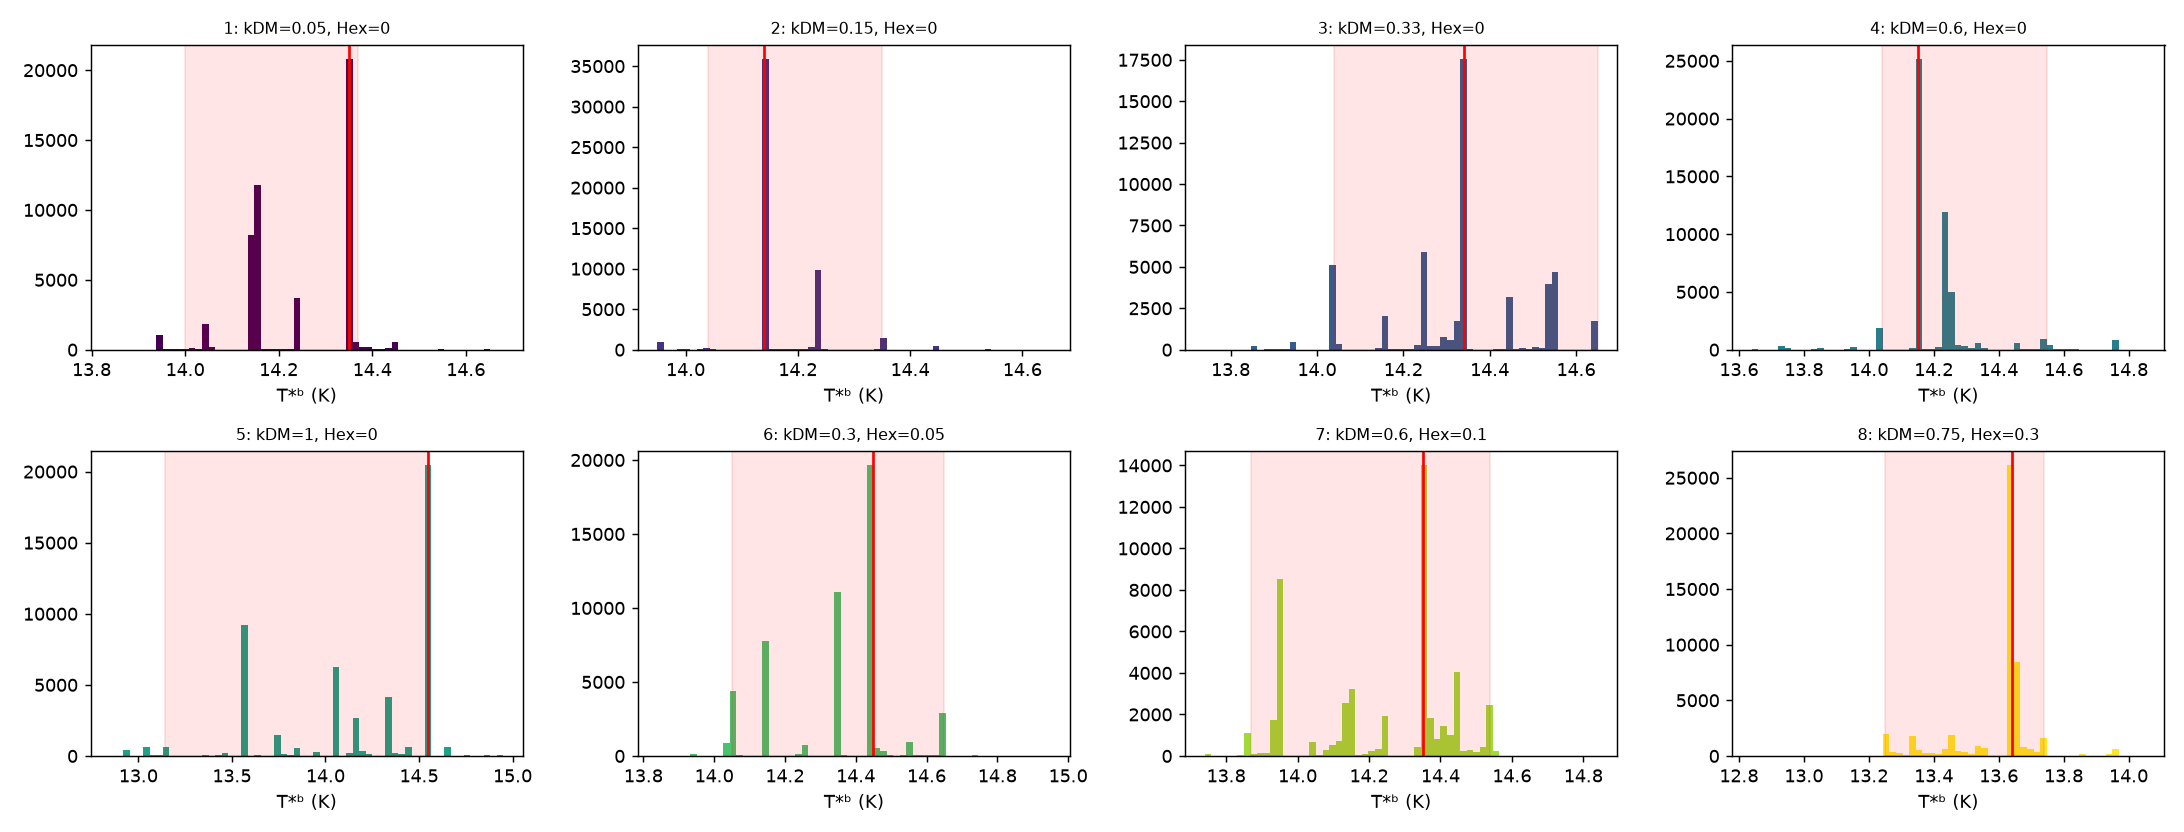
\includegraphics[width=.88\linewidth,height=5.1cm,keepaspectratio]{../informe/latex/fig/T_estrella_bootstrap.png}
\idea{El estado 5 tiene máximos alternativos. El argmax puede saltar entre ellos aunque la altura de la curva cambie poco.}
\fuente{Figura original del informe, 50000 réplicas por caminos. El ajuste BCa es orientativo cuando el argmax es discreto o multimodal.}
\end{frame}

\begin{frame}{Respaldo: jackknife, repesado y EM}
\small
\textbf{Error con dependencia temporal:} omitir bloques contiguos, no observaciones aisladas.
\[
\widehat{\mathrm{se}}_{JK}=\sqrt{\frac{g-1}{g}\sum_{j=1}^{g}(\hat\theta_{(j)}-\bar\theta_{(\cdot)})^2}.
\]
\textbf{Repesado entre temperaturas cercanas:}
\[
\langle A\rangle_\beta\approx\frac{\sum_t A_tw_t}{\sum_t w_t},\qquad w_t=e^{-(\beta-\beta_0)E_t}.
\]
\textbf{EM:} responsabilidades y actualización de las componentes.
\[
r_{jc}=\frac{w_c\phi(\bar m_j;\mu_c,\sigma_c^2)}{\sum_\ell w_\ell\phi(\bar m_j;\mu_\ell,\sigma_\ell^2)},\quad
\mu_c=\frac{\sum_jr_{jc}\bar m_j}{\sum_jr_{jc}},\quad
\mathrm{BIC}=-2\ell+(3k-1)\log100.
\]
\fuente{Se probaron $k=1,2,3$, con 20 arranques por ajuste. El repesado no añade nuevas mediciones independientes.}
\end{frame}

\begin{frame}{Respaldo: sensibilidad del efecto del campo}
\[
\log\tau_m=3.029-2.365\D+2.749H+30.610/T.
\]
\small\renewcommand{\arraystretch}{1.2}
\begin{tabular}{lrrrr}
\toprule
Parámetro & Coeficiente & se HC0 & se agrupado CR1 & Al retirar un estado\\\midrule
$\D$ & $-2.365$&0.072&0.145&[$-2.577,-2.252$]\\
$H$ & 2.749&0.217&0.537&[2.352,6.154]\\
$1/T$ & 30.610&0.792&2.086&[29.476,31.499]\\\bottomrule
\end{tabular}
\idea{Las 141 temperaturas de un estado no son independientes. Con solo ocho grupos y un diseño incompleto, la regresión describe asociaciones y su sensibilidad.}
\small Al excluir el estado 8, el coeficiente de $H$ sube a 6.154. El signo de $\D$ se mantiene al retirar cualquiera de los estados.
\end{frame}

\begin{frame}{Respaldo: diagnóstico al aumentar los barridos}
\grafica{barridos}
\idea{Cerca del máximo, el diagnóstico mejora con la longitud observada. A 6 K puede estancarse. Extrapolar desde 10000 hasta millones de barridos no da una predicción validada.}
\fuente{25 prefijos de medición. Referencias del método: Metropolis et al. (1953); Gelman y Rubin (1992); Vehtari et al. (2021); Efron y Tibshirani (1993); Dempster et al. (1977). Bibliografía completa en el informe.}
\end{frame}

\end{document}
